\icode{E-MD-SI-L3-261120-001}
如图所示，在倾角为\qty{30}{\degree}的光滑斜面上端系有一劲度系数为\qty{75}{N/m}的轻质弹簧，弹簧下端连一个质量为\qty{1}{kg}的小球，球被一垂直于斜面的挡板 \(A\) 挡住。此时弹簧没有形变。若挡板 \(A\) 以\qty{2}{m/s^2}的加速度沿斜面向下做匀加速运动，则\paren[]

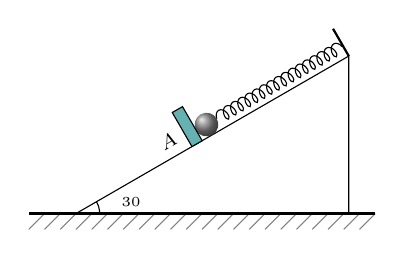
\begin{tikzpicture}[font=\scriptsize]
	\begin{scope}[rotate=30]
		\draw (0,0)--++(4,0)--++(-120:{4*sin(30)});
		\draw[decoration={aspect=.6,segment length=3,amplitude=.8mm,coil},decorate] (2.15,.15)--(4,.15);
		\shade[ball color=gray] (2,.15) circle(.15);
		\draw[fill=teal!60] (1.85,0.5) rectangle(1.7,0)node[above left,rotate=30]{\(A\)};
		\draw[thick] (4,0)--(4,.4);
	\end{scope}
	\draw (.3,0) arc(0:30:.3);
	\node at(.7,.14){\tiny\qty{30}{\degree}};
	\foreach \x in {-.6,-.4,...,3.8}
		\draw[gray] (\x,-.2)--++(.2,.2);
	\draw[thick] (-.6,0)--(3.8,0);
\end{tikzpicture}
\begin{choices}
	\item 开始加速时小球受到挡板的弹力为\qty{5}{N}
	\item 小球向下运动\qty{0.03}{m}时与挡板分离
	\item 小球与挡板分离时的速度为,\qty{0.4}{m/s}
	\item 小球向下运动\qty{0.05}{m}时速度最大
\end{choices}
\begin{answer}
	C\qquad 提示：
\end{answer}